\chapter{Estrategias de Testing}
\label{chap:estrategias-de-testing}

El proceso de testng dentro de un proyecto de software es una actvidad que tene como objetivo \ul{verificar} y \ul{validar} que el software cumple con los requisitos especificados.

El proceso de testing conlleva:
\begin{itemize}
	\item planificación,
	\item diseño,
	\item ejecución de pruebas y
	\item evaluación
\end{itemize}
La gestión de calidad debe garan2zar que el proceso de
testing se lleve a cabo de manera eficiente y eficaz.

\section{Tipos de Testing}
\begin{itemize}
	\item Testeo \textbf{unitario}\\
   Testeo de unidades de software individuales
	\item Testeo de \textbf{integración}\\
   Testeo de los interfaces de y la interacción entre las unidades previamente testeadas
	\item Testeo de \textbf{sistema}\\
   Testeo del sistema entero
	\item Testeo de \textbf{aceptación}\\
   Testeo del sistema y los criterios de aceptación previamente establecidos con el cliente
\end{itemize}

\subsection{Testeo Unitario}
Las \textbf{unidades} son Clases/Métodos (en OO), Procedimientos, Módulos o Componentes. Como se definen las unidades depende del diseño, de la criticidad del software (más crítico implica unidades más pequeñas), de la empresa (estrategia), o del tiempo disponible.


Una \textbf{prueba unitaria} (\texttt{unit test}) es una pieza de código escrita por un desarrollador que pone a prueba un pequeño y específico trozo de código.
Es una manera relativamente barata para mejorar la calidad del código producido, pero \textit{NO} es para usuarios, gerentes, jefes de proyectos: està hech para los programadores.
El programador examina o ejecuta una pequeña
parte de su código, para testear:
\ul{la funcionalidad que él o ella piensa que tiene que tener}

\begin{figure}[htbp]
   \centering
   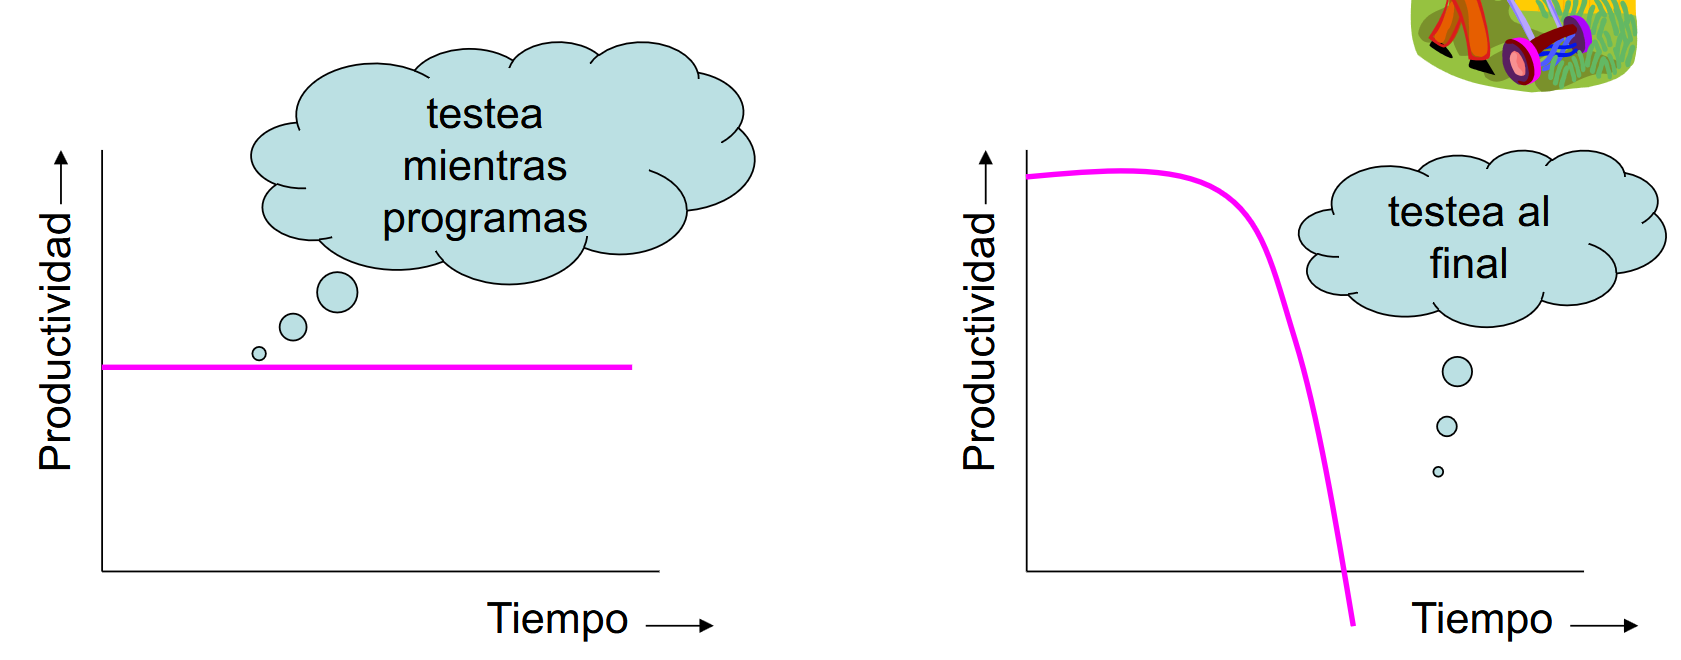
\includegraphics{images/03/unitPostpone.png}
   \caption{Posponer el testeo unitario cuesta mucho tiempo}
   \label{fig:03/unitPostpone}
\end{figure}

\coolquote{
   No es mi trabajo hacer testeo, tenemos un departamento de calidad
}{Bad programmer}

Entonces ¿cuál es el trabajo de un programador? El trabajo de cada programador es \ul{producir código que
funciona y que no contenga ``muchos'' errores}

\subsubsection{JUnit}

\begin{paracol}{2}
	
	\colfill
	JUnit es un framework de testing para Java. JUnit es una herramienta que ayuda a los programadores a escribir pruebas unitarias en Java. JUnit ha sido importante en el desarrollo de la metodología de programación extrema (XP).
	\lstinline|@Test| son los métodos de prueba.
	\begin{itemize}
		\item \lstinline|@BeforeEach| se invoca antes de la ejecución de cada test
		\item \lstinline|@AfterEach| se invoca después de la ejecución de cada test
		\item \lstinline|@BeforeAll| se invoca antes de la ejecución de todos los tests
		\item \lstinline|@AfterAll| se invoca después de la ejecución de todos los tests
	\end{itemize}
	
	\colfill
	\switchcolumn

	\begin{lstlisting}
public class TestDB {
	static private Connection dbConn;
	static private Account acc;
	@BeforeAll
	public static void setUpBeforeAll(){
		dbConn = new Connection("Oracle",15,fred, "f");
		dbConn.connect();
	}
	@AfterAll
	public static void tearDownAfterAll(){
		dbConn.disconnect();
		dbConn = null;
		}
	@BeforeEach
	protected void setUp(){
		acc = new Account();
		}
	@AfterEach
	protected void tearDown(){
		acc = null;
	}
	
	public void testAccountAccess(){
	.../Uses dbConn and acc
	}
	public void testEmployeeAccess(){
		.../Uses dbConn and acc
		}
\end{lstlisting}			
\end{paracol}

\begin{paracol}{2}
	
	\colfill
	En el ejemplo anterior, se muestra un test de una clase \texttt{Account} que tiene una conexión a una base de datos. Se puede ver que se crea una conexión a la base de datos en el método \texttt{setUpBeforeAll} y se cierra en el método \texttt{tearDownAfterAll}. Además, se crea una instancia de la clase \texttt{Account} en el método \texttt{setUp} y se destruye en el método \texttt{tearDown}.
	\colfill
	
	\switchcolumn
	Los metodos son ejecutados en el siguiente orden:
	\ns
	\begin{itemize}
		\item \lstinline|setUpBeforeAll|
		\item \lstinline|setUp|
		\item \lstinline|testAccountAccess|
		\item \lstinline|tearDown|
		\item \lstinline|setUp|
		\item \lstinline|testEmployeeAccess|
		\item \lstinline|tearDown|
		\item \lstinline|tearDownAfterAll|
	\end{itemize}
\end{paracol}

% TODO ejemplo factorial

\subsection{Testeo de Integración}

\begin{definition}
	[Testeo de Integración]
	El testing de las interfaces y la
	interacción entre las unidades previamente testeadas
	mientras que se ensambla el sistema entero
\end{definition}

\begin{itemize}
	\item ¿Qué componentes son el foco del testeo de integración?
	\item ¿En qué orden vamos a testear las interfaces?
	\item ¿Qué técnicas utilizamos para testear las interfaces?
\end{itemize}

Hay tres estrategias:
\begin{enumerate}
	\item \textbf{Big Bang} (todos los componentes a la vez)
	\item \textbf{Bottom-up} (de abajo hacia arriba)
	\item \textbf{Top-down} (de arriba hacia abajo)
\end{enumerate}

\begin{figure}[htbp]
	\centering
	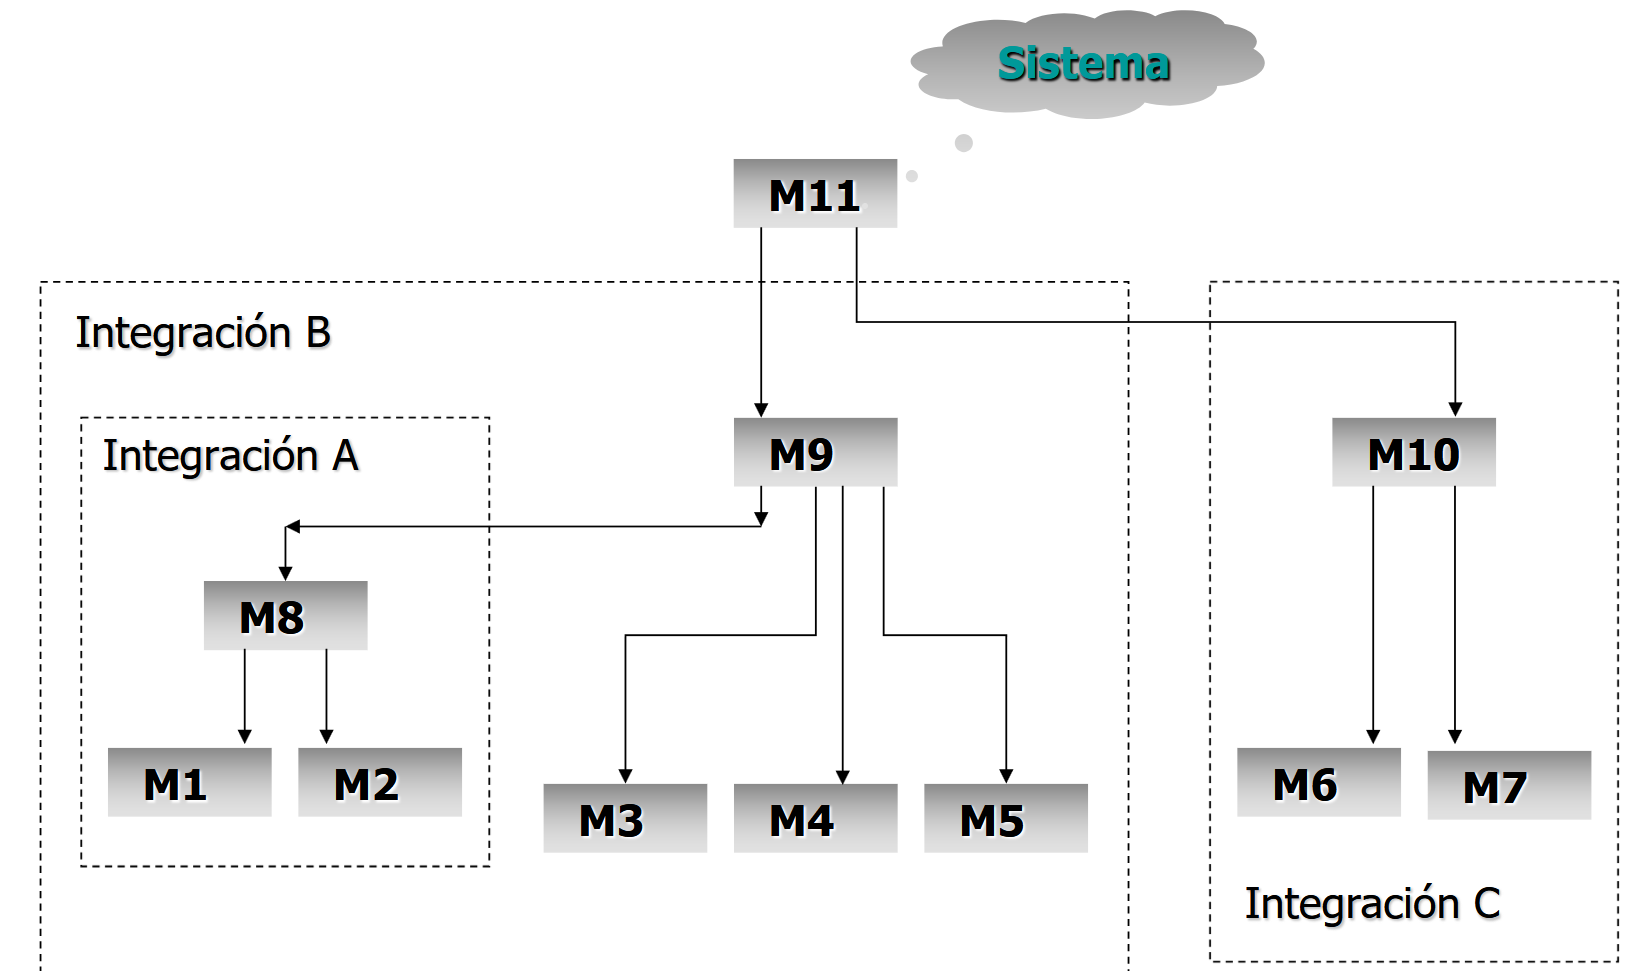
\includegraphics{images/03/bottomup.png}
	\caption{Arbol de dependencia y Bottom-up testing}
	\label{fig:03/bottomup}
\end{figure}

Para hacer el testing \textit{bottom-up} necesitamos \textbf{drivers}.
Un driver es un programa que invoca un componente bajo testeo, por ejemplo, para simular un componente de un nivel superior cuyo código todavía no está disponible (está todavía en desarrollo).

\begin{figure}[htbp]
	\centering
	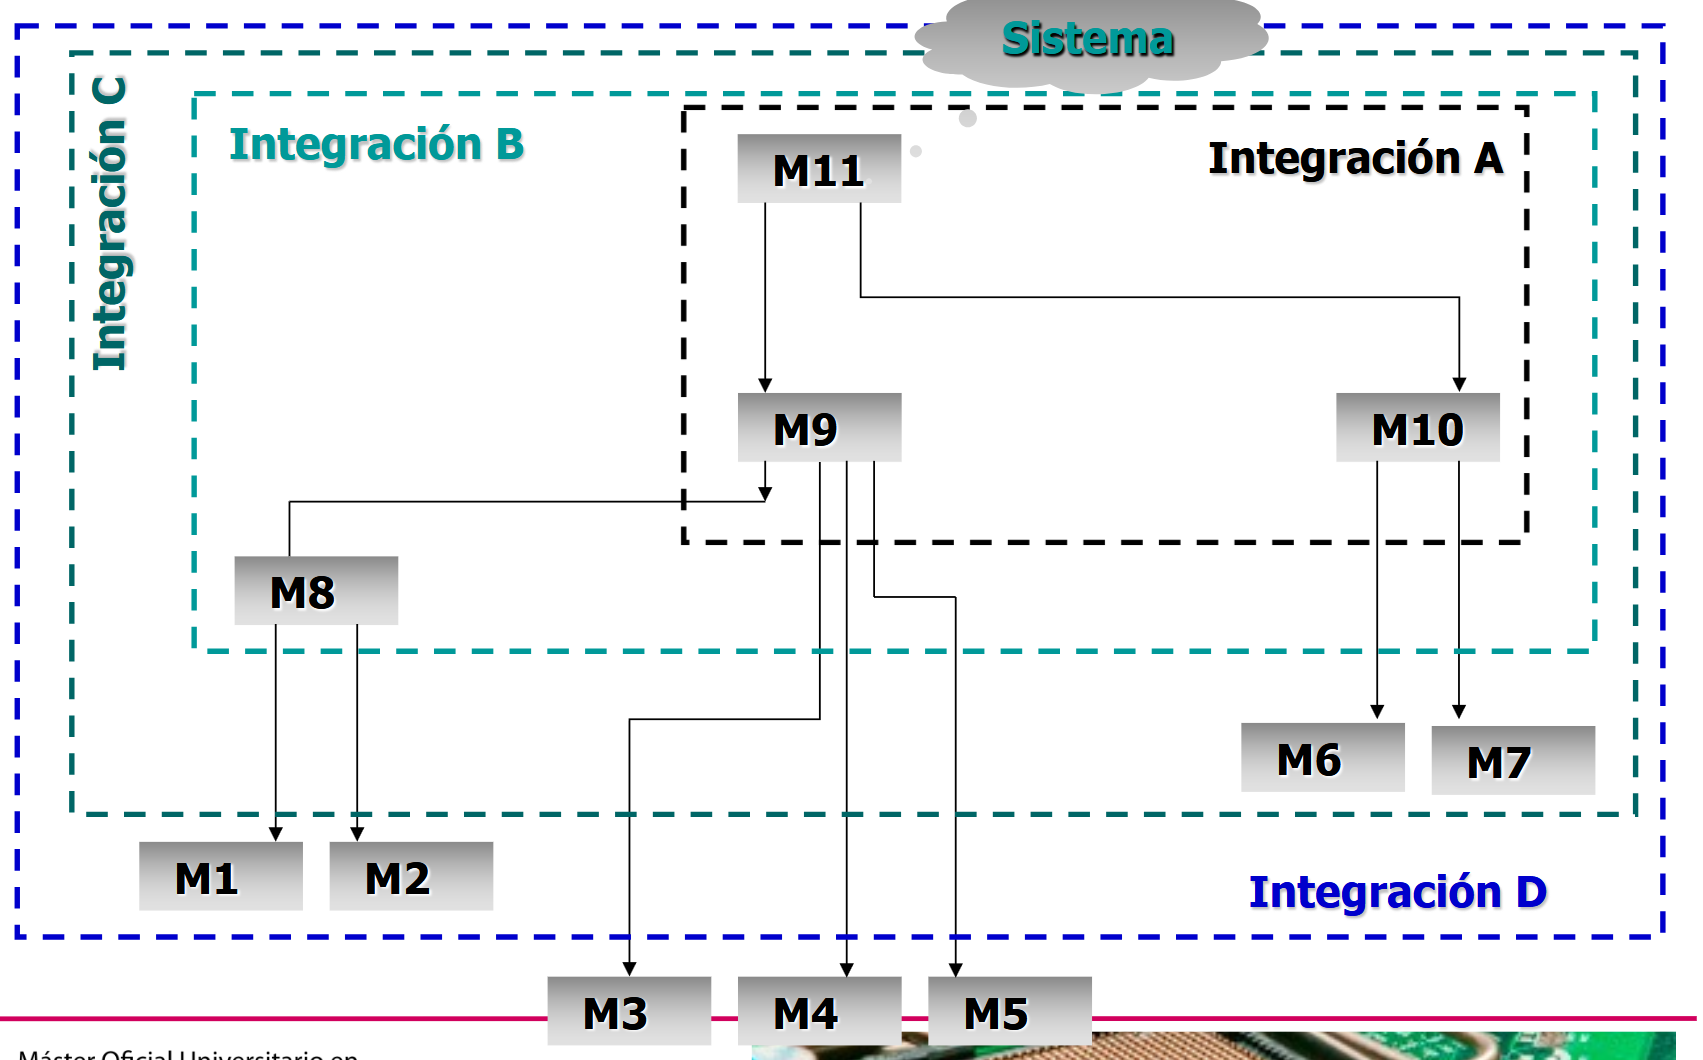
\includegraphics{images/03/topdown.png}
	\caption{Top-down testing}
	\label{fig:03/topdown}
\end{figure}

Para hacer el testeo de integración de manera \textit{top-down}, se
necesita dobles, que simulan componentes de un nivel inferior (``Stub'', ``dummy'', ``fake'', ``mock'').
\ns

El \textit{Big Bang} testing se utiliza solo para sistemas pequeños, ya que es muy difícil de manejar en sistemas grandes.


\subsubsection{Mockito}
Mockito es un framework de testing para Java que permite crear objetos simulados (mocks) de clases y interfaces. Mockito se utiliza para simular objetos que son necesarios para realizar pruebas unitarias. Se puede integrar con JUnit para realizar pruebas unitarias en Java. 
En las slides se muestran ejemplos de cómo utilizar Mockito.

Mockito es muy comodo para implementar el testeo de integración de manera \textit{top-down}.
% TODO Parte 2 y 3	

\section{Testeo de Sistema}
Se verifica que se cumple los requisitos especificados, es decir, que el sistema realiza correctamente todas las funcionesque se han detallado en las especificaciones dadas por el usuario del sistema.

Es necesario automatizar las prubas, y por esto se utilizan herramientas como \textit{Selenium}, que permite automatizar pruebas en navegadores web: en este caso, hablamos de pruebas de \textbf{funcionalidad}.

Para testar el \textbf{rendimiento} (tiempo de respuesta, carga, memoria.) se utilizan herramientas como \textit{JMeter} o \textit{NeoLoader}.

Otros aspectos importantes que el testeo debe cubrir son \textbf{Seguridad} y \textbf{Usabilidad}.

\section{Testeo de aceptación}
Esto testeo es dirigido a los criterios de aceptación
previamente establecidos con el cliente. Se puede hacer de manera manual o automatizada.

\subsection{Regresión}
Testeo que se necesita hacer después de cambios en el
software para asegurar que no se ha introducido defectos.

\ul{El testeo de \textbf{regresión} se tiene que automatizar} por el simple hecho de que el testeo de regresión manual \textit{NO SE HACE}.

\section{Gestión de Defectos, métricas y mas}

{El proceso de clasificación de defectos incluye tres fases:\ns
\begin{enumerate}
	\item Detección de defectos
	\item Investigación de defectos
	\item Resolución de defectos
\end{enumerate}}

\note{
\begin{itemize}
	\item \textbf{Actividad} (que estábamos haciendo cuando encontramos el fallo)
	\item \textbf{Fase del proyecto} (en que estábamos cuando encontramos el fallo)
	\item \textbf{Repetitividad} (¿se puede repetir el error?)
	\item \textbf{Síntoma} (fallo del sistema, mensaje de error, entrada no aceptado, resultado
incorrecto, etc.)
	\item \textbf{Causa} (nuestro producto, componente externo, usuario, etc.)
	\item \textbf{Origen} (especificación de requisitos, diseño, programación, etc.)
	\item \textbf{Impacto} (misión: crítico, medio, …; en la planificación; para el cliente, etc.)
\end{itemize}
}

\subsection{Métricas}


 Las métricas son observaciones cuantitativas para:
\begin{itemize}
	\item Informar sobre el \textbf{progreso del proyecto} de testeo
\note{\begin{itemize}
	\item ¿Qué tareas han terminado en tiempo?
	\item ¿Qué tareas han terminado antes?
	\item ¿Qué tareas han tenido retraso?
	\item ¿Cómo vamos siguiendo la planificación?
	\item Si no vamos bien, ¿cuáles son las razones?
	\item ¿Qué productividad ha tenido persona/equipo X?
\end{itemize}}
	\item Informar sobre la \textbf{calidad del software}
	\note{\begin{itemize}
		\item ¿Podemos parar el testeo?
	\item ¿Podemos entregar producto?
	\item ¿Hemos resueltos todos los defectos?
	\item ¿Cómo estamos gesHonando los defectos?
	\item ¿Cuántos defectos hemos encontrado por: subsistema,
	origen, causa, severidad, etc\dots?
	\end{itemize}}
	\item Informar sobre la \textbf{calidad del testeo}
	\note{\begin{itemize}
		\item ¿Estamos haciendo los tests necesarios?
		\item ¿Están siendo efectivos los tests?
		\item ¿Estamos utilizando los casos de prueba adecuados?
		\item ¿Necesitamos tener en cuenta diferentes casos de prueba?
	\end{itemize}}
\end{itemize}

La cobertura del testeo es una métrica importante para evaluar la calidad del testeo. La cobertura del testeo es la medida de la cantidad de código que ha sido ejecutado por los tests, especialmente en lo que se refiere a instrucciones, decisiones y condiciones (múltiples).\\
Pero puede referirse también a la cobertura de los requisitos, de los casos de uso, de los casos de prueba, etc.

\begin{lstlisting}[caption={Con 1 test donde \lstinline|x==y| se cubre todo el codigo, pero no todas las decisiones. En efecto, el defecto ocurre cuando \lstinline|x!=y|}]
	int foo_3 ( ) {
		int* p = NULL;
		int x;
		if (x==y) {
			p = &x;
		}
		*p = 123;
	}
\end{lstlisting}

\subsection{Mutación}

La mutación es una técnica de testing que consiste en introducir errores en el código fuente para ver si los tests son capaces de detectarlos. Se puede utilizar para evaluar la calidad de los tests.

\subsection{Organización del testing}
Se puede dedicar un equipo de testo integrado, con un jefe, o se puede haber que desarrolladores y testeadores son las mismas personas y no hay testeadores a tiempo completo.
La ventaja de tener un equipo de testeo es que se puede tener una visión más objetiva del software, ya que los testeadores no han desarrollado el software; al contrario, si los desarrolladores hacen el testeo, no tienen que comunicar con los testeadores, y conocen el software.

Otra tecnica de organización es \textit{Outsourcing}, que consiste en contratar una empresa externa para hacer el testeo. La ventaja es que se puede tener una visión más objetiva del software, y se puede tener acceso a expertos en testeo. La desventaja es que se puede tener problemas de comunicación, y que se puede tener problemas de confidencialidad.

